\begin{figure*}

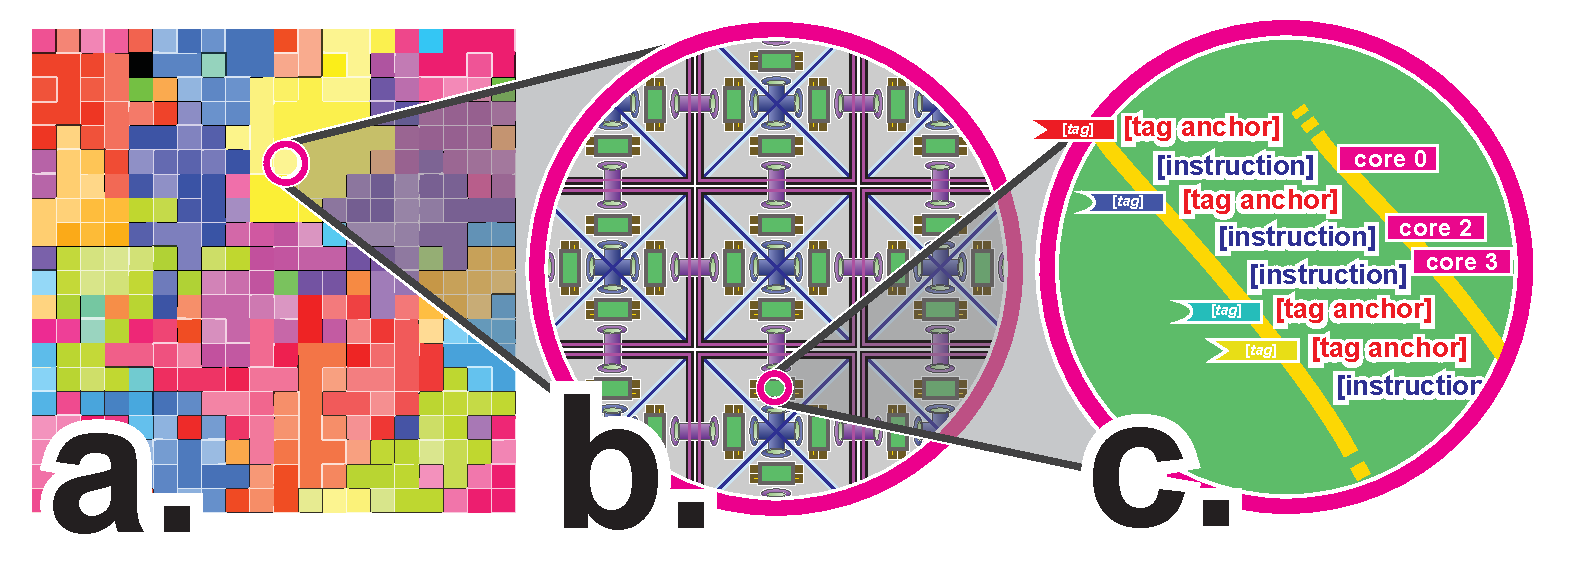
\includegraphics[width=\linewidth]{{img/overview}}

\caption{ \footnotesize
Overview of DISHTINY system.
Cells occupy slots on a toroidal grid (Subfigure $a$).
As cells reproduce, they may grow their existing kin group (shown here by color) or splinter off to found new ones.
Each cell, shown here bounded within black squares, is controlled by four virtual CPUs, referred to as ``cardinals'' and shown here within triangles (Subfigure $b$).
Cardinals within a cell can interact via message passing (blue conduits).
Cardinals can interact with the corresponding cardinal in their neighboring cell through message passing or simulation intrinsics (i.e., resource sharing, offspring spawning, etc.), represented here by purple conduits.
These inter-cell interactions may span physical hardware threads or processes.
All virtual CPUs within a cell independently execute the same linear genetic program (Subfigure $c$).
Tagged subsections of this linear genetic program (``modules'') activate in response to stimuli.
}
\label{fig:overview}
\end{figure*}
